\section{Motion detection}
In this section we will discuss the analysis of a scene, not only in terms of a static image, but also in terms of temporal evolution of it.
\textbf{Motion} is one of the most important features of a scene, and we are usually interested in detecting:
\begin{itemize}
    \item \textbf{Moving objects}, which are the objects that are moving in the scene;
    \item \textbf{Camera motion}, which is the motion of the camera itself.
\end{itemize}

Motion can be formally defined as the change of position of an object in a scene over time. In the 3D case, 
it can be represented as:
\begin{equation}
    \boldsymbol{D}(\boldsymbol{X}, t_1, t_2) = \boldsymbol{X'} - \boldsymbol{X} = [\Delta x, \Delta y, \Delta z]
\end{equation}
When projected into the 2D image plane we get:
\begin{equation}
    \boldsymbol{d}(\boldsymbol{x}, t_1, t_2) = \boldsymbol{x'} - \boldsymbol{x} = [\Delta x, \Delta y]
\end{equation}
\begin{figure}[H]
    \centering
    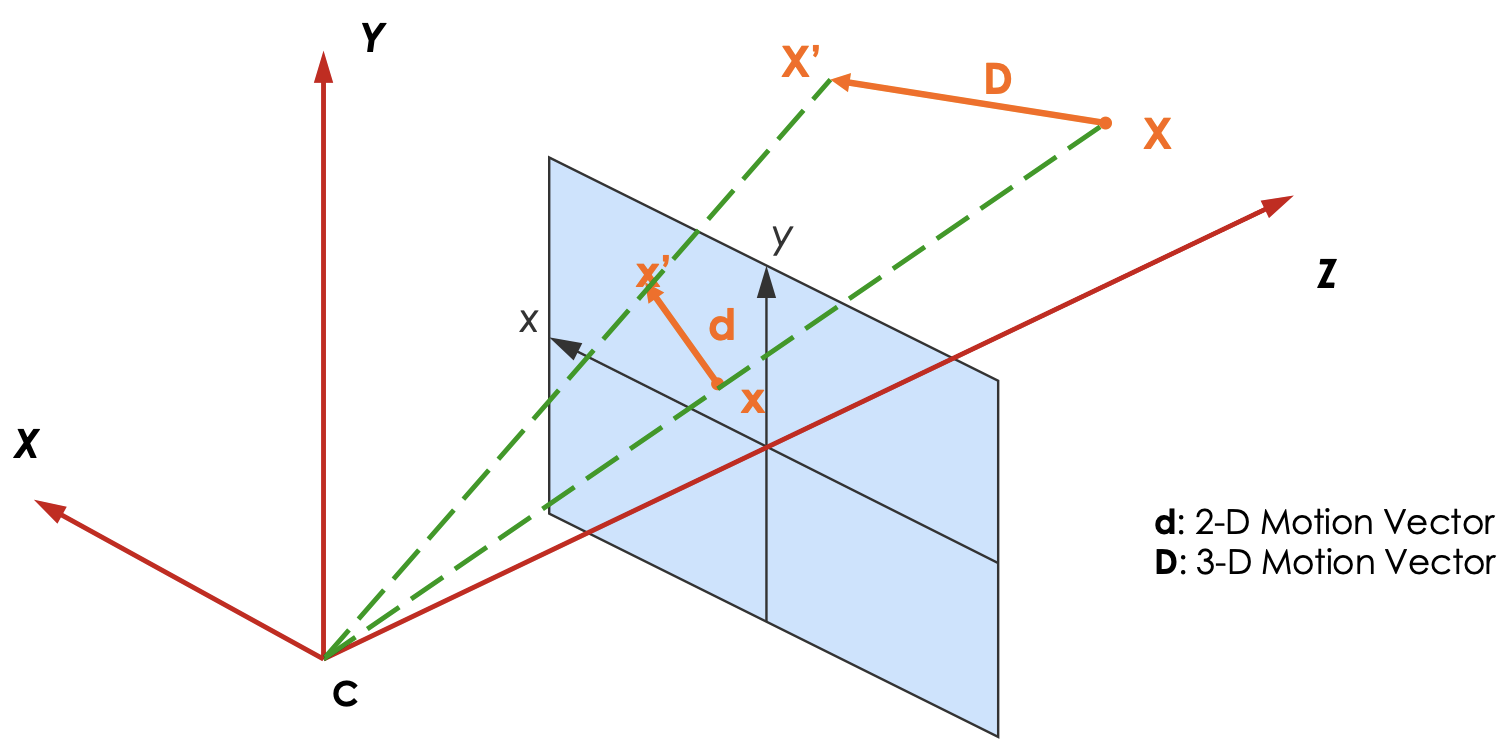
\includegraphics[width=0.7\textwidth]{media/motion-detection/projection.png}
    \caption{Projection of movement from 3D to 2D.}
\end{figure}
From this, if we consider a single point, we can derive that the displacement we perceive in the image plane can be quite different from the actual 3D displacement, 
due to the projection of the 3D scene onto the 2D image plane.

The final goal of the analysis of motion is to be able to extract the \textbf{motion field}, which is the set of all the displacements of all the points in the scene,
understand if it really corresponds to the actual motion of the objects in the scene, and understand if it was caused by the motion of the camera itself or by the motion of the objects in the scene.

\paragraph{An example}
\begin{figure}[H]
    \centering
    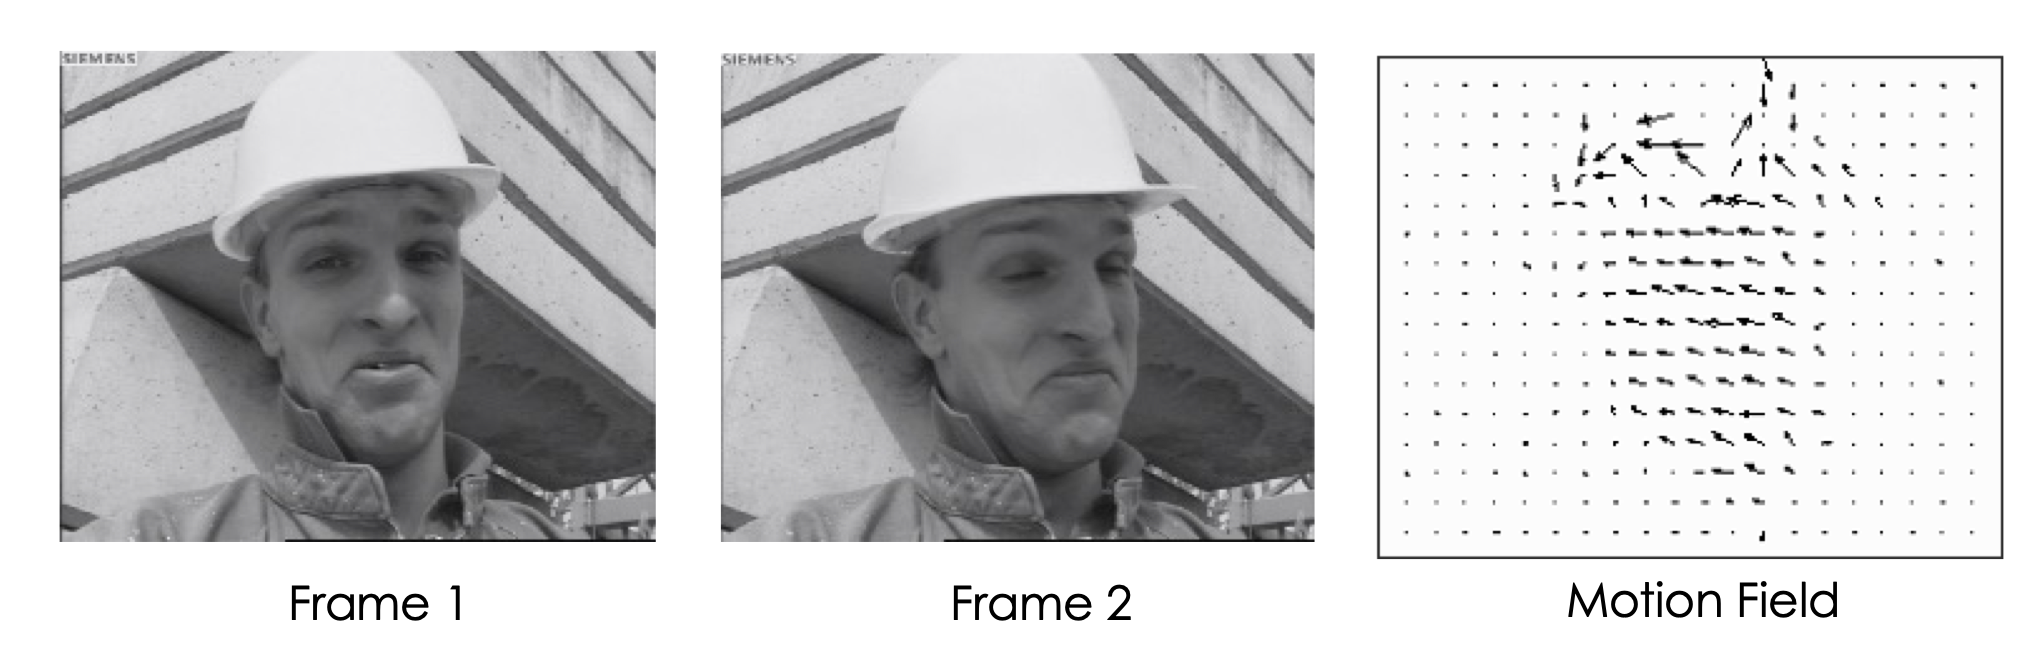
\includegraphics[width=0.7\textwidth]{media/motion-detection/example.png}
    \caption{Example of motion detection.}
\end{figure}
In this example, we can clearly identify three main components of the motion field:
\begin{itemize}
    \item The motion of the face, which moved from left to right between the two frames. In fact, in the \textbf{motion field},
    we can see the arrows pointing from left, as signaling that the "point" of frame 2 is to the right of the corresponding "point" in frame 1.
    \item Static section, corresponding to the background, which is not moving, and therefore has no motion field. If arrows were present,
    they would represent the motion of the camera, as the background of this example is static;
    \item The motion of the head. Since the safety helmet is mostly flat, the algorithm is not able to correctly identify the motion of the head. In the motion field, this results
    in a "noisy" motion field, with arrows pointing in different directions, and not corresponding to the actual motion of the head.
\end{itemize}

\paragraph{Applications}
Motion detection is a fundamental task in computer vision, and it has many applications, such as:
\begin{itemize}
    \item \textbf{Detection of moving objects}, which is useful for surveillance, traffic monitoring, and many other applications;
    \item \textbf{Segmentation of moving objects};
    \item \textbf{Recognition}, we could filter different objects based on their motion (e.g., we could recognize a car from a pedestrian based on their motion);
    \item \textbf{Filtering};
    \item \textbf{Compression}, in case of videos, the motion component can be used to compress the video.
\end{itemize}
In general, it is used to detect changes of the image intensity, in the scene over time.

\subsection{Problems}
The motion detection task is quite challenging, and the solution might be \textbf{not unique}.

In fact, the motion is based on the \textbf{velocity} of the points in the scene, over two frames. This might not reflect the actual motion of the objects in the scene,
as it might also be caused by \textbf{camera motion} or by \textbf{illumination changes}.

\subsubsection{Real vs Apparent movement}
Also, being the motion perceived by changes in the scene, we could have two possible situations for which the motion field is not reflecting the actual motion of the objects in the scene:
\begin{itemize}
    \item \textbf{Constant illumination}, in which a sphere is moving in the scene (rotating around its own axis), but the illumination is constant.
    In this case, the motion field will be zero, as there are no changes in the image intensity, even though the sphere is moving.
    \item \textbf{Changing illumination}, in which the sphere is not moving, but the illumination source rotates around the sphere. 
    In this case, the motion field will be non-zero, as there are changes in the image intensity, even though the sphere is not moving.
\end{itemize}

\subsubsection{Occlusion}
Another non-trivial problem is the occlusion. This problem occurs when an object in the background is partially or completely occluded by an object in the foreground.
This can cause problems in the motion detection, as a static background might be perceived as moving, due to the occlusion of the foreground object.
\begin{figure}[H]
    \centering
    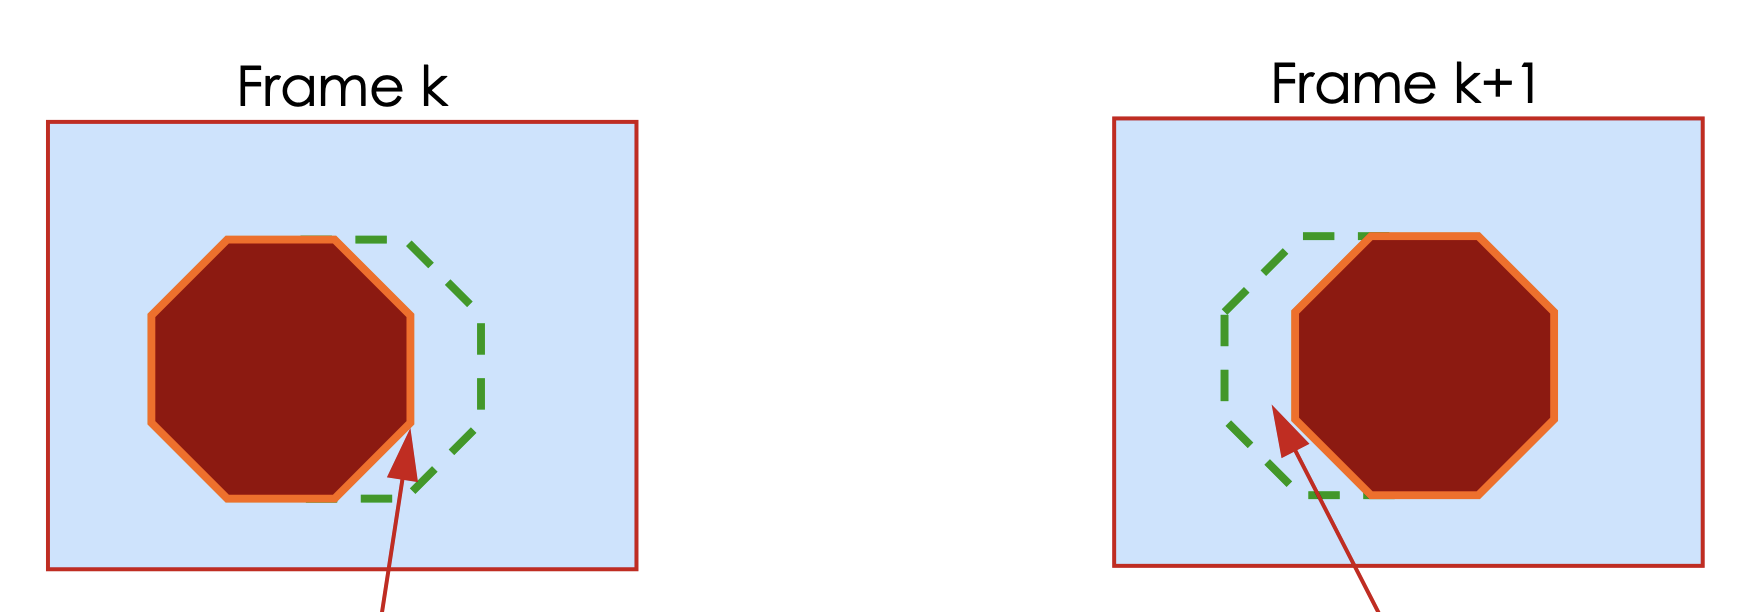
\includegraphics[width=0.7\textwidth]{media/motion-detection/occlusion.png}
    \caption{Example of occlusion.} 
\end{figure}

\subsubsection{Aperture}
Not all motion can be detected by analyzing the changes in the image intensity. In fact, only displacements
of the borders of the objects can be detected, while the motion of the internal points of the objects cannot be detected.

Also, borders can only detect the motion in the direction perpendicular to the border itself (in the direction of the intensity gradient), 
while for angles, we can detect motion in both directions.

\subsection{Optical Flow}
The motion detection we have described so far can be formalized trough the concept of \textbf{optical flow}.

First, we define the assumption taken in the optical flow:
\begin{itemize}
    \item \textbf{Brightness constancy}: the object illumination does not change over time;
    \item \textbf{Small motion}: the motion between two frames is small enough;
    \item \textbf{Spatial coherence}: each point $[x, y]$ in the image plane is shifted to a new position $[x + \Delta x, y + \Delta y]$.
    This impose that the motion is only a translation, and that there is no rotation or scaling.
\end{itemize}
This is usually not true in real scenarios, but it is a good approximation for small motions.

\subsubsection{Optical Flow Function}
The optical flow function is defined as:
\begin{equation}
    \label{eq:optical_flow}
    \psi(x + \Delta x, y + \Delta y, t + \Delta t) = \psi(x, y, t)
\end{equation}
This means that the intensity of the point $[x, y]$ at time $t$ is the same as the intensity of the point $[x + \Delta x, y + \Delta y]$ at time $t + \Delta t$,
as long as the motion is small enough. This is the brightness constancy assumption.

The Taylor expansion states that for a function $f(x + \Delta x)$, we can approximate it as:
\begin{equation*}
    f(x + \Delta x) \approx f(x) + \frac{\partial f}{\partial x} \Delta x
\end{equation*}
By applying the Taylor expansion to the left-hand side of the equation \ref{eq:optical_flow}, we get:
\begin{equation*}
    \psi(x + \Delta x, y + \Delta y, t + \Delta t) \approx \psi(x, y, t) + \frac{\partial \psi}{\partial x} \Delta x + \frac{\partial \psi}{\partial y} \Delta y + \frac{\partial \psi}{\partial t} \Delta t
\end{equation*}
By substituting this into the equation \ref{eq:optical_flow}, we get:
\begin{equation*}
    \frac{\partial \psi}{\partial x} \Delta x + \frac{\partial \psi}{\partial y} \Delta y + \frac{\partial \psi}{\partial t} \Delta t = 0
\end{equation*}
By dividing both sides by $\Delta t$, we get:
\begin{equation*}
    \frac{\partial \psi}{\partial x} \frac{\Delta x}{\Delta t} + \frac{\partial \psi}{\partial y} \frac{\Delta y}{\Delta t} + \frac{\partial \psi}{\partial t} = 0
\end{equation*}
By defining the velocity of the point as $v_x = \frac{\Delta x}{\Delta t}$ and $v_y = \frac{\Delta y}{\Delta t}$, we get the optical flow equation:
\begin{equation}
    \frac{\partial \psi}{\partial x} v_x + \frac{\partial \psi}{\partial y} v_y + \frac{\partial \psi}{\partial t} = 0
\end{equation}
This implies that the variation of the intensity of a point in the image plane is related to the velocity of the point in the image plane. 

If we decompose the velocity into its components (normal and tangential with respect to the surface of the object),
we can see that only the normal component of the velocity can be detected, since the tangential component does not cause any change in the intensity of the point. 
This is the aperture problem we have discussed before.

\subsection{Motion Detection in practice}
There are two main approaches to motion detection in practice:
\begin{itemize}
    \item \textbf{Intensity-based methods}, which are based on the analysis of the changes in the image intensity over time;
    \item \textbf{Feature-based methods}: based on the analysis of the changes in the features of the objects in the scene over time.
    This requires additional steps of feature extraction and matching, but it can be more robust to changes in the illumination and to occlusions.
\end{itemize}

\subsubsection{Change Detection}
The change detection is a simple approach to motion detection. 
It takes as input two frames of a video, taken at different time instants, and it computes the difference between the two frames.
This can be done by simply following the following steps:
\begin{itemize}
    \item \textbf{Subtraction}: we compute the difference between the two frames, pixel by pixel.
    The resulting image will have high intensity values in the areas where there is a change in the intensity, and low intensity values in the areas where there is no change.
    \item \textbf{Thresholding}: we apply a threshold to the resulting image, to obtain a binary image. The pixels with intensity values above the threshold
    will be set to 1, and the pixels with intensity values below the threshold will be set to 0.
\end{itemize}
From a computational point of view, this approach is very simple and fast. We can formalize it as:
\begin{itemize}
    \item \textbf{Frame difference}: corresponds to the subtraction of two images $I_K - I_{K-1}$.
    We can define the \textbf{frame differencing operation} as:
    \begin{equation}
    \label{eq:frame_difference}
        FD_{K, K-1}(x, y) = s(x, y, k) - s(x, y, k-1)
    \end{equation}
    If $FD$ is not null, then a change has been detected in the pixel $[x, y]$;
    \item \textbf{Tresholding}: to filter out the noise, we can apply a threshold to the resulting image. We can define the \textbf{thresholding operation} as:
    \begin{equation}    
        \label{eq:thresholding}
        T(x, y) = \begin{cases}
            1 & \text{if } FD_{K, K-1}(x, y) > \tau \\
            0 & \text{otherwise}
        \end{cases}
    \end{equation}
\end{itemize}
This algorithm allows to quickly adapts to changes in the backgrounds and to the stopping of the moving objects.
It can detect the contours of the moving objects, but it is not able to detect the motion of the internal points of the objects, due to the aperture problem.

To resolve these problems, usually the time scale of the analysis is increased, by considering more distant frames. 
This allows to detect the motion of the internal points, but for fast moving objects, it can cause problems.

\subsubsection{Background subtraction}
The background subtraction is a more sophisticated approach to motion detection. 
It is based on the idea of modeling the background of the scene as a static image (acquired a priori).

The algorithm can be formalized as follows:
\begin{algorithm}
    \caption{Background subtraction algorithm}
    \label{alg:bg_subtraction}
    \begin{algorithmic}[1]
        \State $B = I(0)$; \Comment{Initialize background model}
        \For{each frame $I(t)$}
            \State $D = |I(t) - B|$; \Comment{Difference between current frame and background}
            \State $M = Threshold(D)$; \Comment{Apply thresholding to obtain the motion mask}
        \EndFor
    \end{algorithmic}
\end{algorithm}
This allows for a better representation of the moving objects in the scene, as it can filter out the static background, 
but it has a few limitations, such as:
\begin{itemize}
    \item \textbf{Modelling the background}: the background model might not be accurate, especially in case of dynamic backgrounds;
    \item \textbf{Changes in the background}: if a background object starts moving, both the real object and its "ghost" will be detected as moving objects;
    \item \textbf{Illumination changes}: if the illumination changes, the background model is not able to adapt to it as it is based on a static image;
    \item \textbf{Camera motion}: if the camera is moving, again the background model is not able to adapt to it.
\end{itemize}

\subsubsection{Adaptive Background Subtraction}
To overcome the limitations of the background subtraction, we can use an adaptive background subtraction approach.
In this approach, the background model is updated over time, to adapt to changes in the background and to changes in the illumination.
The update of the background model can be formalized as:
\begin{equation}
    B_t = \alpha I(t) + (1 - \alpha) B_{t-1}
\end{equation}
Where $\alpha$ is a parameter that controls the update rate of the background model:
\begin{itemize}
    \item If $\alpha$ is close to 1, the background model will be updated quickly, going back to the \textbf{change detection} approach;
    \item If $\alpha$ is close to 0, the background model will be updated slowly, maintaining a more stable representation of the background.
\end{itemize}

\subsubsection{Gaussian Average}
Instead of relying on a single background model, we can use a Gaussian Model to represent the background.
In this approach, we model the background as a Gaussian distribution, and we update the parameters of the distribution over time,
with the same approach of the adaptive background subtraction. 

We can formalize the Gaussian model as follows:
\begin{equation}
    \label{eq:gaussian_update}
    \mu_t = \alpha I_t + (1 - \alpha) \mu_{t-1}
\end{equation}
This model can adapt to changes in the background and to changes in the illumination,
by "absorbing" the changes in the background into the parameters of the Gaussian distribution.
The speed of adaptation is controlled by the parameter $\alpha$, as in the adaptive background subtraction approach.

This model allows recognizing the moving objects in the scene, even in case of dynamic backgrounds.
We can instead say that a pixel belongs to the foreground if the intensity value of the pixel is far from the mean of the Gaussian distribution, by a certain threshold:
\begin{equation}
    |I_t - \mu_t| > k \sigma_t
\end{equation}
Where $k$ is the threshold parameter, and $\sigma_t$ is the standard deviation of the Gaussian distribution at time $t$.

Even though the model is constantly updated, usually an initialization phase is required, in which the background model is learned from a sequence of frames. This allows to have a more accurate
representation of the background, and to reduce the number of false positives in the motion detection.

\subsubsection{Improving the Gaussian Average}
From the equation \ref{eq:gaussian_update} of the Gaussian average, we can see that the update of the mean is based on both
background and foreground pixels, with no distinction between them.

To avoid foreground pixels to affect the update of the background model, we can use a \textbf{selective update} approach,
in which only the pixels that are classified as background are used to update the background model. This can be formalized as:
\begin{equation}
    \mu_t = M\mu_{t-1} + (1 - M)(\alpha I_t + (1 - \alpha) \mu_{t-1})
\end{equation}
Where $M$ is a binary mask that indicates which pixels are classified as background (1) and which pixels are classified as foreground (0).
If the pixel is classified as foreground, the background model is not updated at all, while if the pixel is classified as background, 
the background model is updated as in the Gaussian average approach.

\subsubsection{Mixture of Gaussian}
There are cases in which a single Gaussian distribution is not enough to model the background. For example,
in case of rain, snow, or waving trees, the background can have multiple modes, and a single Gaussian distribution is not able to capture all the variations in the background.
These are known as multimodal backgrounds, and they require a more complex model to be able to capture all the variations in the background.

In this case, we can use a mixture of Gaussian distributions to model the background.
In particular, we can model the background as a mixture of $K$ Gaussian distributions, where each distribution represents a different mode of the background.
More formally, we can define the mixture of Gaussian model as:
\begin{equation}
    P(X_t) = \sum_{i=1}^{K} w_{i,t} \mathcal{N}(X_t | \mu_i, \Sigma_i)
\end{equation}
Where:
\begin{itemize}
    \item $P(X_t)$ is the probability of the pixel intensity $X_t$ at time $t$;
    \item $w_{i,t}$ is the weight of the $i$-th Gaussian distribution at time $t$, which represents the importance of the $i$-th mode of the background at time $t$;
    \item $\mathcal{N}(X_t | \mu_i, \Sigma_i)$ is the Gaussian distribution with mean $\mu_i$ and covariance $\Sigma_i$.
\end{itemize}
By assuming that each color channel is independent, we can simplify the model by using a diagonal covariance matrix, which reduces the number of parameters to be estimated.

\paragraph{Identify each Distribution}
Once we have defined the $K$ Gaussian distributions, we need to rank them based on their weights $w_{i,t}$, amplitude and standard deviation, to determine which distributions represent the background and which distributions represent the foreground.
Usually, the distributions with the highest weights and lowest standard deviation are considered as background distributions, while the distributions with the lowest weights and highest standard deviation are considered as foreground distributions.
Formally, the first $B$ distributions that satisfy the following condition are considered as background distributions:
\begin{equation}
    \sum_{i=1}^{B} w_{i,t} > T
\end{equation}
Where $T$ is a threshold parameter that controls the sensitivity of the model to changes in the background.

\paragraph{Point classification}
Given the mixture of Gaussian model, we can check each pixel intensity $X_t$ against the distributions:
\begin{itemize}
    \item If $X_t$ matches one of distributions, it is classified accodingly.
    $X_t$ is said to match a distribution if the distance between $X_t$ and the mean of the distribution is less than a certain threshold:
    \begin{equation*}
        |X_t - \mu_i| < k \sigma_i
    \end{equation*}
    \item If $X_t$ does not match any of the distributions, the distribution with the lowest weight is replaced
    with a new distribution with mean equal to $X_t$, high standard deviation, and low weight.
\end{itemize}

\paragraph{Update Model parameters}
Also in this case, the parameters of the model are updated over time, to adapt to changes in the background and to changes in the illumination.
In particular, we are interested in updating the weights of the distributions, since the means and the standard deviations are updated just as in the 
Gaussian average approach, but only for the distribution that matches the pixel intensity $X_t$.

The update of the weights can be formalized as:
\begin{equation}
    w_{i,t} = (1 - \alpha) w_{i,t-1} + \alpha M
\end{equation}
Where $M$ is a binary variable that indicates whether the distribution matches the pixel intensity $X_t$ (1 if it matches, 0 otherwise).
This update allows to increase the weight of the distribution that matches the pixel intensity $X_t$, 
and to decrease the weight of the distributions that do not match the pixel intensity $X_t$.